%%%%%%%%%%%%%%%%%%%%%%%%%%%%%%%%%%%%%%%%%%%%%%%%%%%
%
%  New template code for TAMU Theses and Dissertations starting Fall 2016.  
%
%
%  Author: Sean Zachary Roberson
%  Version 3.17.09
%  Last Updated: 9/21/2017
%
%%%%%%%%%%%%%%%%%%%%%%%%%%%%%%%%%%%%%%%%%%%%%%%%%%%
%%%%%%%%%%%%%%%%%%%%%%%%%%%%%%%%%%%%%%%%%%%%%%%%%%%%%%%%%%%%%%%%%%%%%%
%%                           TIME TO SOLUTION ESTIMATOR CHAPTER
%%%%%%%%%%%%%%%%%%%%%%%%%%%%%%%%%%%%%%%%%%%%%%%%%%%%%%%%%%%%%%%%%%%%%



\chapter{TIME-TO-SOLUTION ESTIMATOR \label{cha:tts}}

Before optimization of the partitioning scheme can occur, it is necessary to have an estimation tool that gives the approximate sweep time for a given partitioning scheme. The time-to-solution estimator serves as the objective function that gets optimized, with the partitions serving as the parameter space. This chapter will detail the time-to-solution estimator, and showcase the results of 2D and 3D verification studies. 

The time to solution estimator is written in Python 3. Python was chosen as the language because of it's powerful graph library, networkx. 
This library gives us a wide variety of graph mathematics that is optimized and easy to use. 

\section{Method}
The time-to-solution estimator determines the time to sweep across a domain by:
\begin{enumerate}
	\item Given a partitioning scheme, build adjacency matrices.
	\item Build Directed Acyclic Graphs  (DAGs) from the adjacency matrices, one for each quadrant/octant.
	\item Determine the cells per subset and boundary cells per subset for the given mesh.
	\item Weight the edges of each graph based on the solve and communication time of each subset to its neighbors.
	\item Adjust the weights of each graph to operate on the universal timescale.
	\item Adjust the weights of each graph to accommodate angular pipelining.
	\item Adjust the weights of each graph to reflect sweep conflicts between octants. 
	\item Calculate the time to solution.
\end{enumerate}

\subsection{Building the adjacency matrices}

Before building the graph for each quadrant/octant, an adjacency matrix must be built for the given partitioning scheme. 
The adjacency building process relies on a major assumption: The z dimension has partitions all the way across the domain, then the x dimension has partitions per plane, then the y dimension has partitions per plane per column. 
In future work, these three dimensions will be interchangeable, but for now, this ordering must be preserved. The adjacency building algorithm differs slightly for 2D and 3D cases. Both are detailed in the following subsection. 

\subsubsection{2D adjacency matrices}

To build the adjacency matrices in 2 dimensions, we only need the partitioning scheme.

\subsubsection{3D adjacency matrices}

\subsection{Building the directed acyclic graphs (DAGs)}

The adjacency matrices give us crucial connectivity information in order to build our graphs. This process also slightly from 2D to 3D.

\subsubsection{2D graph building}
In two dimensions, we build four graphs corresponding to four quadrants. 
We define the quadrants in the following manner:
\begin{itemize}
  \item Quadrant 0: $\Omega_x > 0$, $\Omega_y > 0$
  \item Quadrant 1: $\Omega_x > 0$, $\Omega_y < 0$
  \item Quadrant 2: $\Omega_x < 0$, $\Omega_y > 0$
  \item Quadrant 3: $\Omega_x < 0$, $\Omega_y < 0$
\end{itemize}


\subsubsection{3D graph building}


\section{2D Verification}

A verification study in 2D was run to verify the time-to-solution estimator for 2D partitioning schemes with perfectly balanced partitions. The test problems were verified against a code written by Jean Ragusa that mimics PDT's scheduler in two dimensions. For consistency, the time-to-solution estimator utilized an unweighted depth-of-graph algorithm during the verification study to match PDT's scheduling. The verification study consists of the following problems:
\begin{enumerate}
	\item 2x2 to 10x10 subsets in x and y with regular partitions and 1 to 6 angles per quadrant.
	\item 2x2 to 10x10 subsets in x and y with mildly random partitions and 1 to 6 angles per quadrant.
	\item  2x2 to 10x10 subsets in x and y with random partitions and 1 to 6 angles per quadrant.
	\item  2x2 to 10x10 subsets in x and y with probable worst-case partitions and 1 to 6 angles per quadrant.
\end{enumerate}

"Mildly random" partitions keep the cut lines uniformly distributed in x, while the y cut lines vary slightly around the uniformly distributed cut lines of the regular partitions. Figure \ref{mild_random_partitions} shows examples of this partitioning style. "Random" partitions possesses no such limitations on either set of cut lines, as shown by Fig. \ref{random_partitions}. 

Figures \ref{regular_partitions}, \ref{mild_random_partitions}, \ref{random_partitions}, \ref{worst_partitions} show the four partitioning schemes and Figs. \ref{regular_verification}, \ref{mild_random_verification}, \ref{random_verification}, \ref{worst_verification} show the results of the verification study for each partitioning scheme. In the results, a stage is defined as the time it takes to solve all cells in a subset for an angle.  

\subsection{Regular Partitions}

Figure \ref{regular_partitions} shows four examples of the regular partitioning scheme used for the first part of the verification study. Cut lines in both dimensions go all the way across the domain. This reflects the partitioning scheme after the original load balancing algorithm described in Section \ref{sec:og_lb} is used.

%Regular partitions
\begin{figure}[H]
\centering
\begin{subfigure}[b]{0.45\textwidth}
  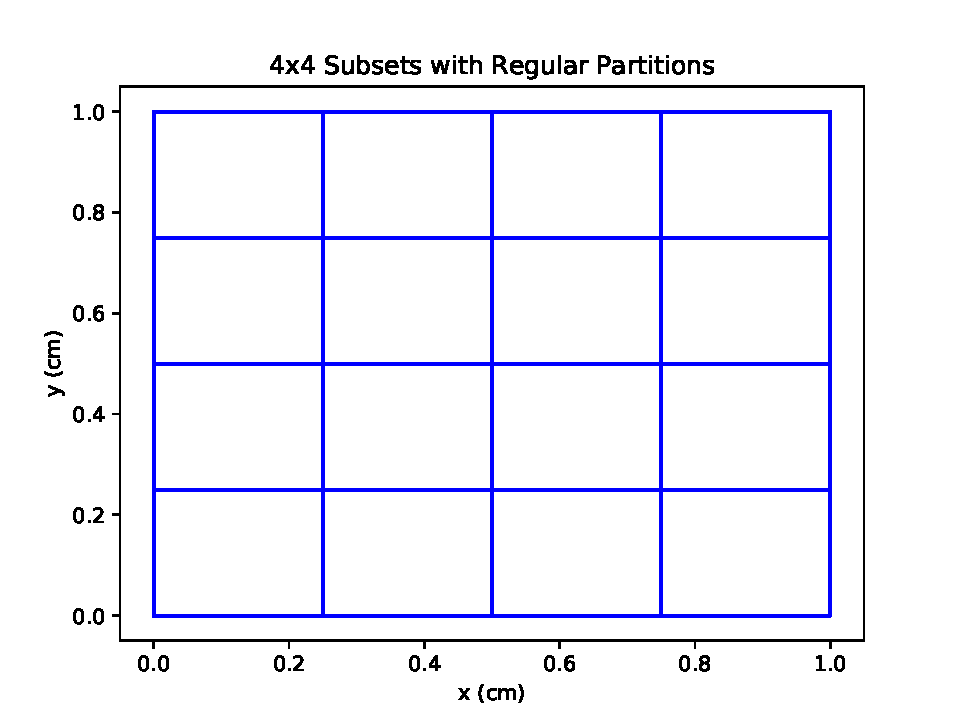
\includegraphics[width=\textwidth]{../cut_line_files/4_regular.pdf}
  \caption{4x4 subsets with regular partitions.}
  \label{4regular}
\end{subfigure}
\begin{subfigure}[b]{0.45\textwidth}
  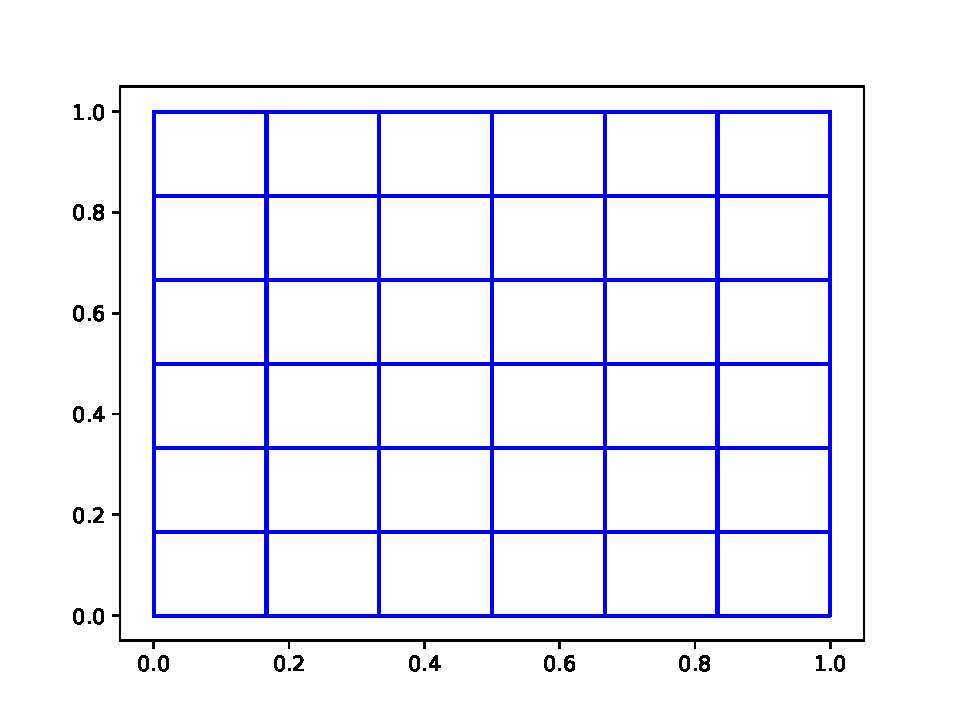
\includegraphics[width=\textwidth]{../cut_line_files/6_regular.pdf}
  \caption{6x6 subsets with regular partitions.}
  \label{6regular}
\end{subfigure}

\begin{subfigure}[b]{0.45\textwidth}
  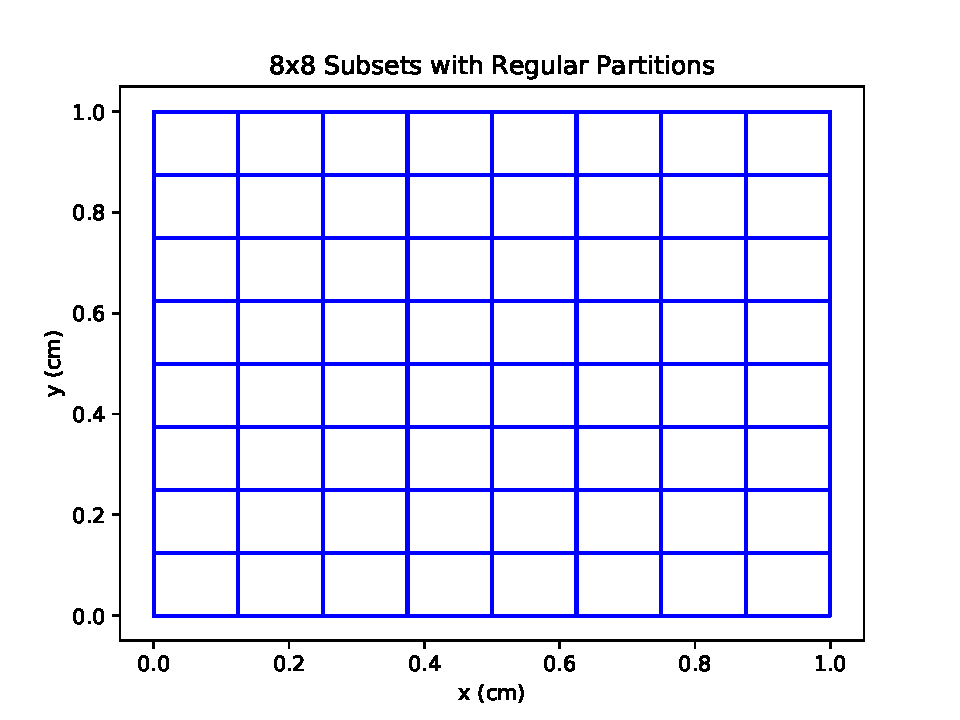
\includegraphics[width=\textwidth]{../cut_line_files/8_regular.pdf}
  \caption{8x8 subsets with regular partitions.}
  \label{8regular}
\end{subfigure}
\begin{subfigure}[b]{0.45\textwidth}
  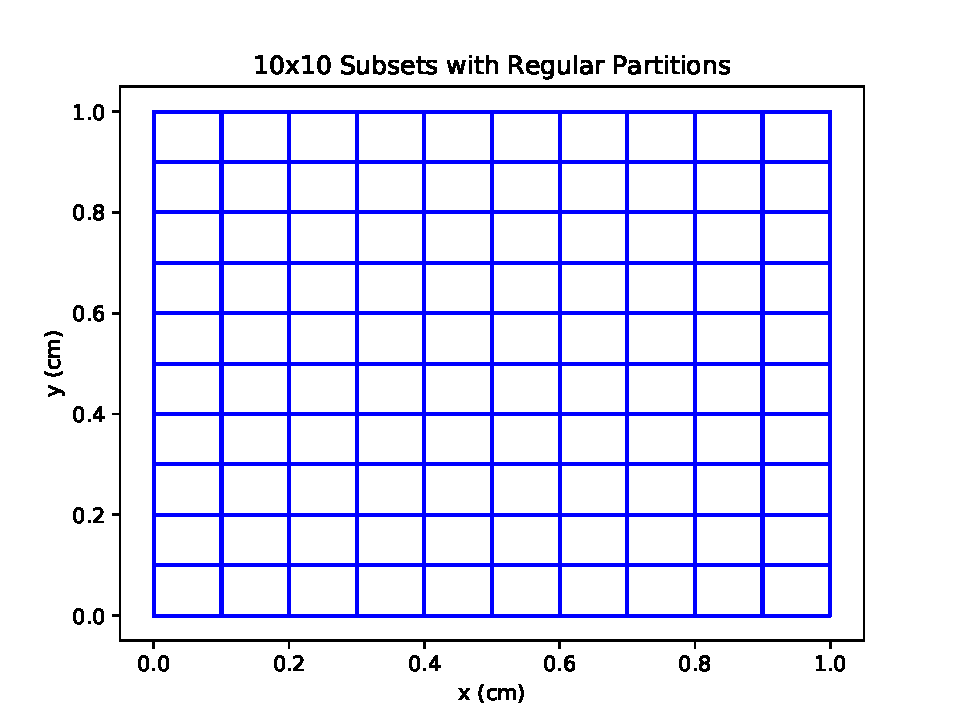
\includegraphics[width=\textwidth]{../cut_line_files/10_regular.pdf}
  \caption{10x10 subsets with regular partitions.}
  \label{10regular}
\end{subfigure}
\caption{Examples of regular partitioning.}
\label{regular_partitions}
\end{figure}

Using regular partitions as shown in Fig. \ref{regular_partitions}, the first portion of the 2D verification study was run from 2x2 to 10x10 subsets in x and y and 1 to 6 angles per quadrant.  Figure \ref{regular_verification} shows the results of the time-to-solution estimator (solid line) against Ragusa's code (points) for each test case. The time-to-solution estimator verifies perfectly on regular partitions with multiple angles per quadrant. 

%Verification plots.
\begin{figure}[H]
\centering
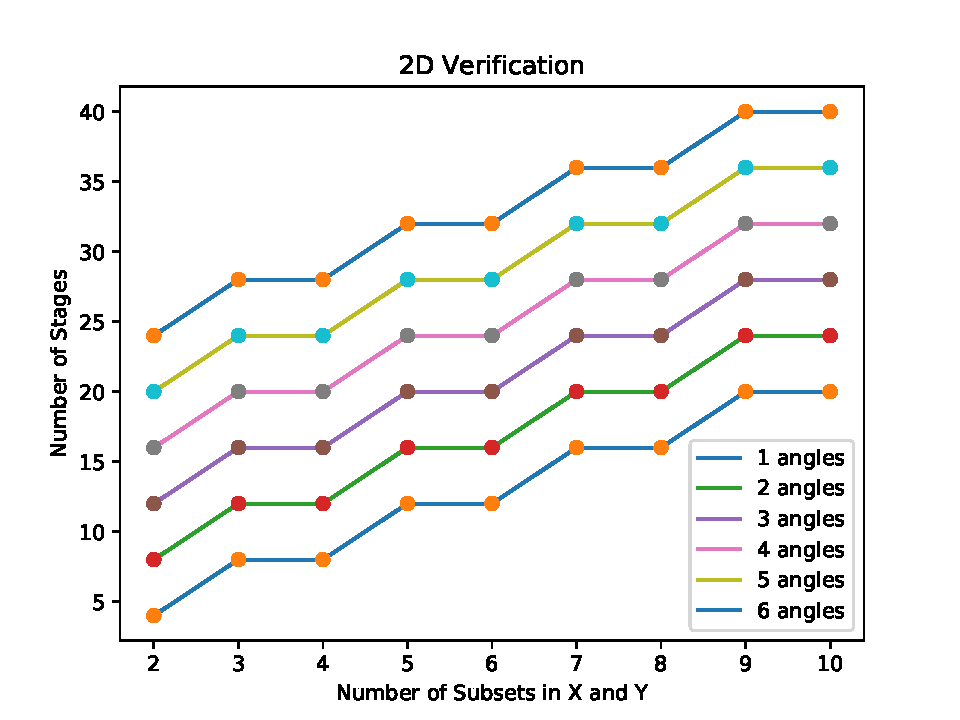
\includegraphics[scale=0.8]{../figures/regular_verification.pdf}
\caption{A 2D verification suite with regular partitions run from 2x2 to 10x10 subsets with each case being run from 1 to 6 angles per quadrant.}
\label{regular_verification}
\end{figure}

\subsection{Mildly Random Partitions}
Figure \ref{mild_random_partitions} shows four examples of the mildly random partitioning scheme used for the second part of the verification study. Cut lines in the x dimension go all the way across the domain, and are uniformly distributed. This reflects a possible partitioning scheme after the load balancing by dimension algorithm described in Section \ref{sec:lbd} is used.

%Mild random partitions
\begin{figure}[H]
\centering
\begin{subfigure}[b]{0.45\textwidth}
  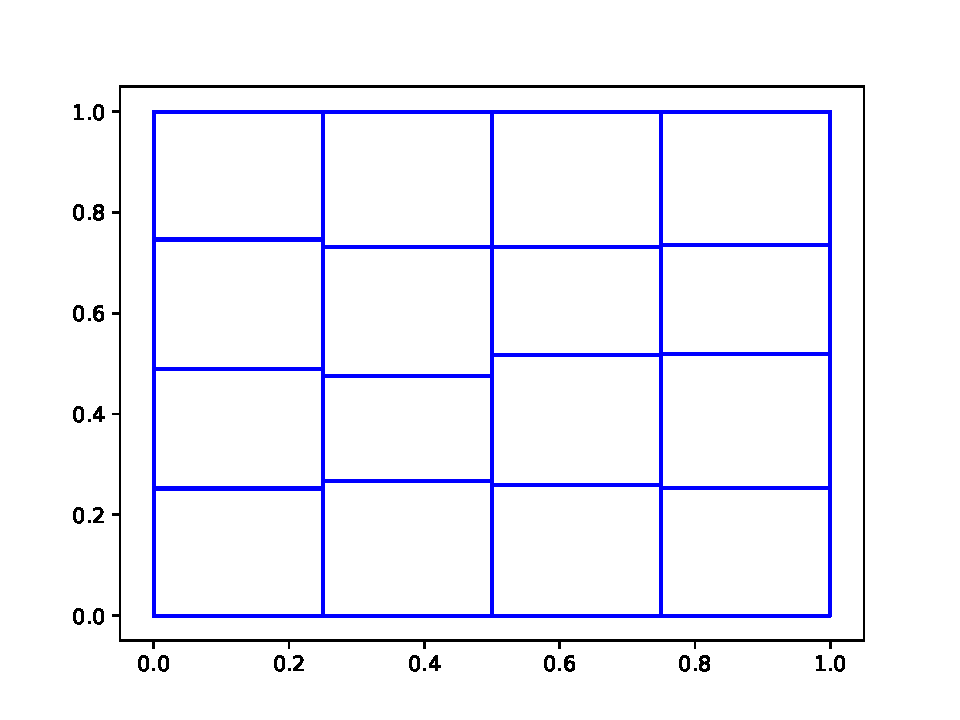
\includegraphics[width=\textwidth]{../cut_line_files/4_mild_random.pdf}
  \caption{4x4 subsets with mildly random partitions.}
  \label{4mildrandom}
\end{subfigure}
\begin{subfigure}[b]{0.45\textwidth}
  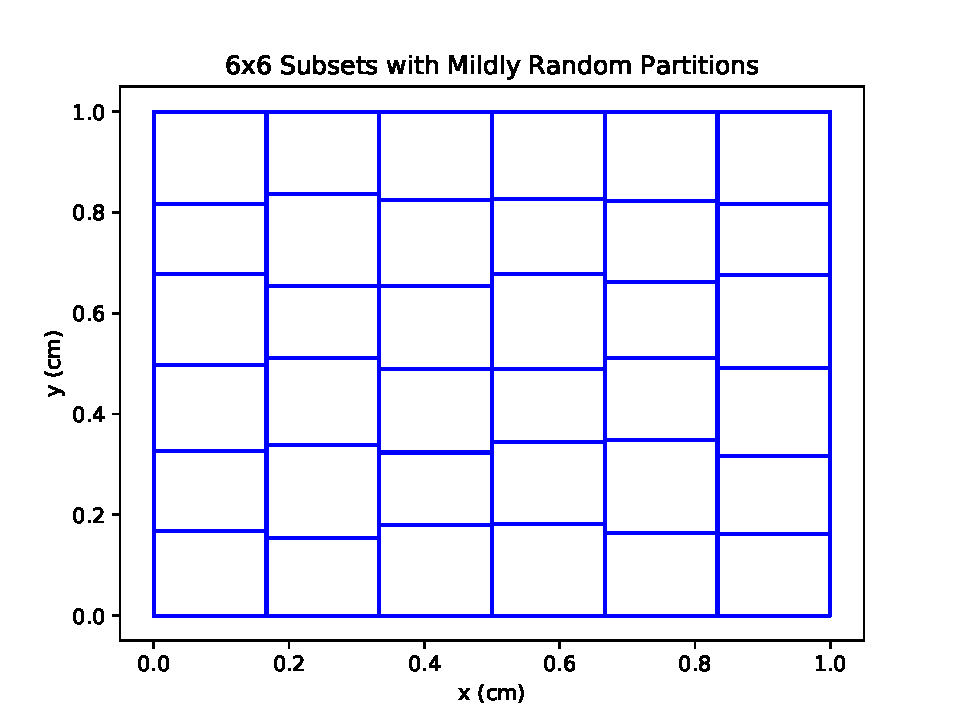
\includegraphics[width=\textwidth]{../cut_line_files/6_mild_random.pdf}
  \caption{6x6 subsets with mildly random partitions.}
  \label{6mildrandom}
\end{subfigure}

\begin{subfigure}[b]{0.45\textwidth}
  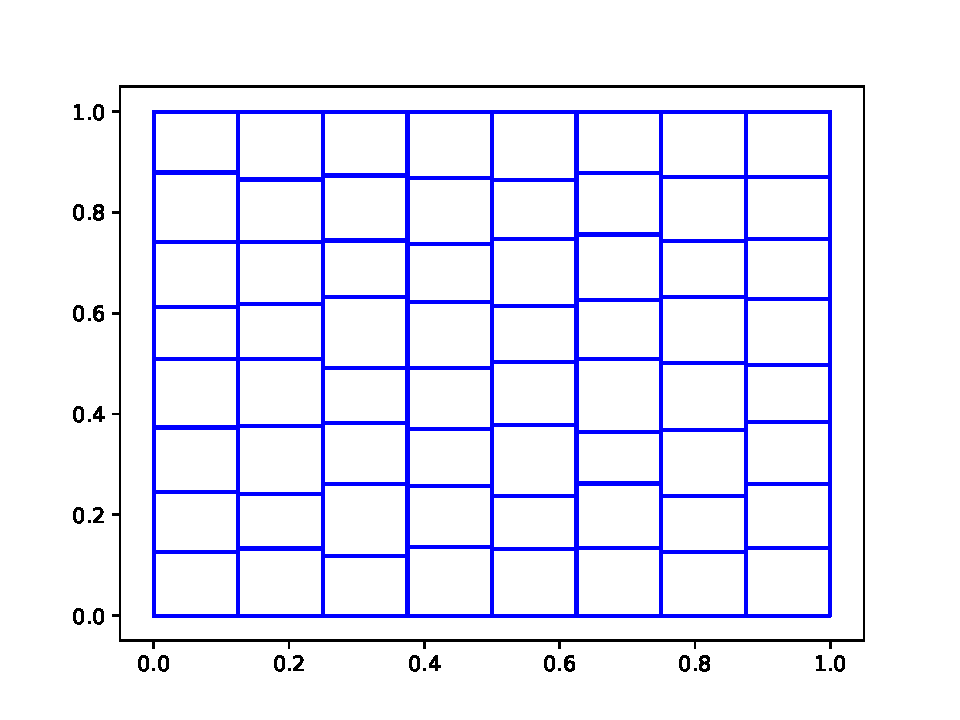
\includegraphics[width=\textwidth]{../cut_line_files/8_mild_random.pdf}
  \caption{8x8 subsets with mildly random partitions.}
  \label{8mildrandom}
\end{subfigure}
\begin{subfigure}[b]{0.45\textwidth}
  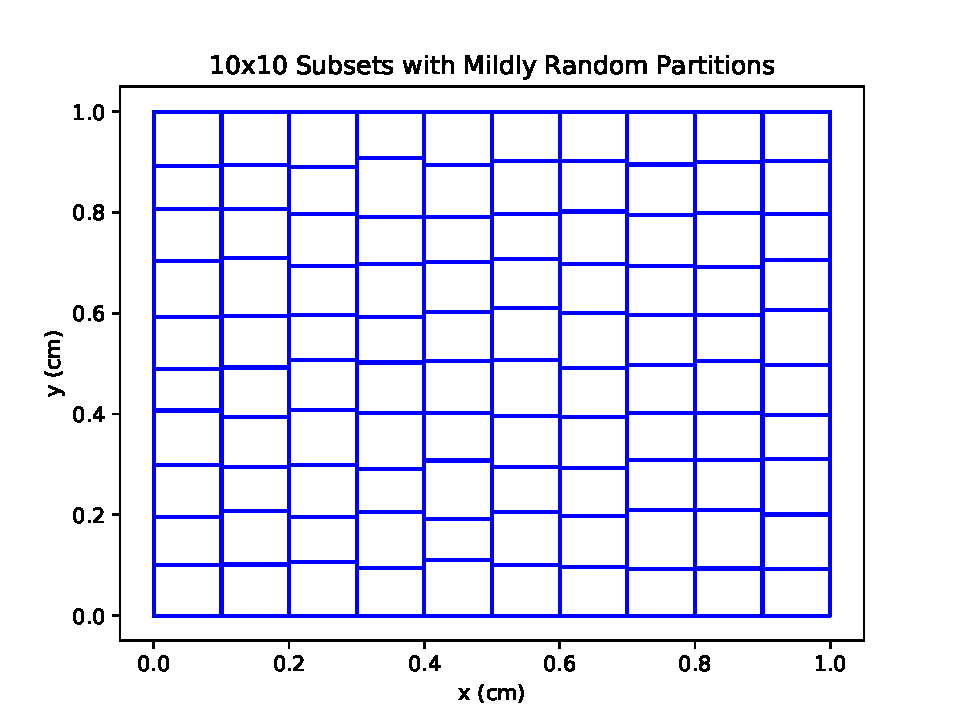
\includegraphics[width=\textwidth]{../cut_line_files/10_mild_random.pdf}
  \caption{10x10 subsets with mildly random partitions.}
  \label{10mildrandom}
\end{subfigure}
\caption{Examples of mildly random partitioning.}
\label{mild_random_partitions}
\end{figure}

Using mildly random partitions as shown in Fig. \ref{mild_random_partitions}, the second portion of the 2D verification study was run from 2x2 to 10x10 subsets in x and y and 1 to 6 angles per quadrant.  Figure \ref{mild_random_verification} shows the results of the time-to-solution estimator (solid line) against Ragusa's code (points) for each test case. The time-to-solution estimator verifies perfectly on mildly random partitions with multiple angles per quadrant. 

\begin{figure}[H]
\centering
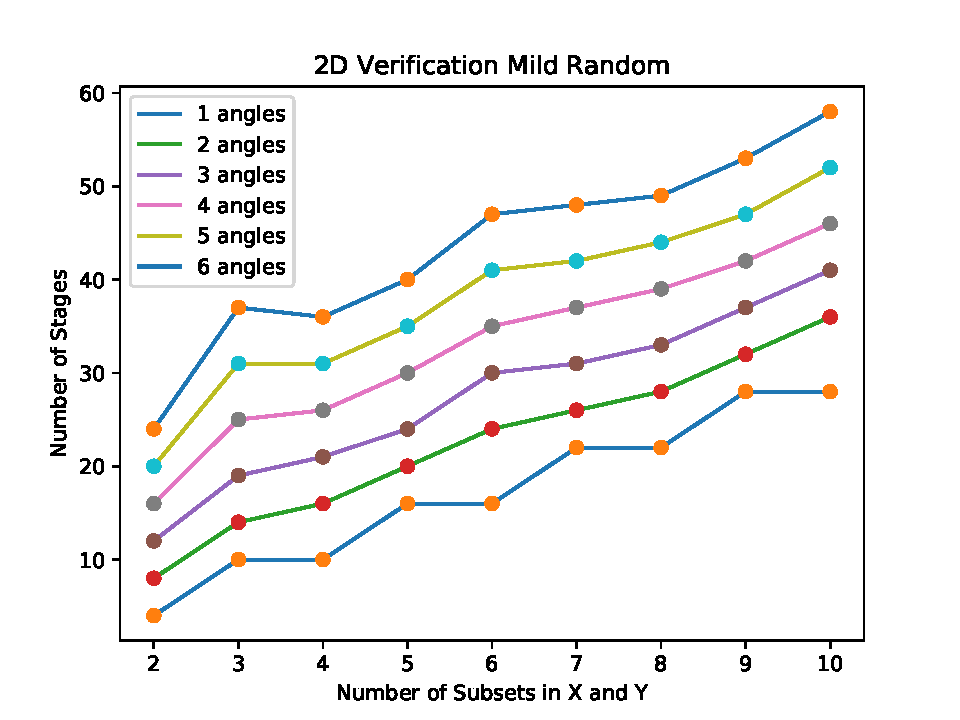
\includegraphics[scale=0.8]{../figures/mild_random_verification.pdf}
\caption{A 2D verification suite with mildly random partitions run from 2x2 to 10x10 subsets with each case being run from 1 to 6 angles per quadrant.}
\label{mild_random_verification}
\end{figure}

\subsection{Random Partitions}
%Random partitions
Figure \ref{random_partitions} shows four examples of the random partitioning scheme used for the third part of the verification study. Cut lines in the x dimension go all the way across the domain, but are not necessarily uniformly distributed. The cut lines in y are randomly distributed in each column.This reflects a possible partitioning scheme after the load balancing by dimension algorithm described in Section \ref{sec:lbd} is used.
\begin{figure}[H]
\centering
\begin{subfigure}[b]{0.45\textwidth}
  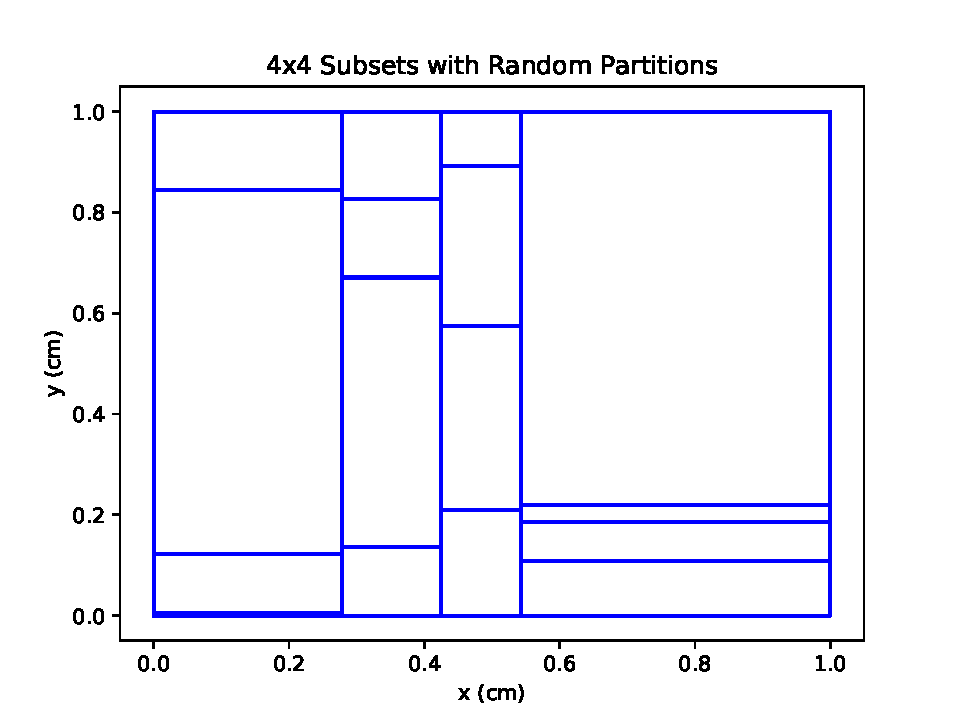
\includegraphics[width=\textwidth]{../cut_line_files/4_random.pdf}
  \caption{4x4 subsets with random partitions.}
  \label{4random}
\end{subfigure}
\begin{subfigure}[b]{0.45\textwidth}
  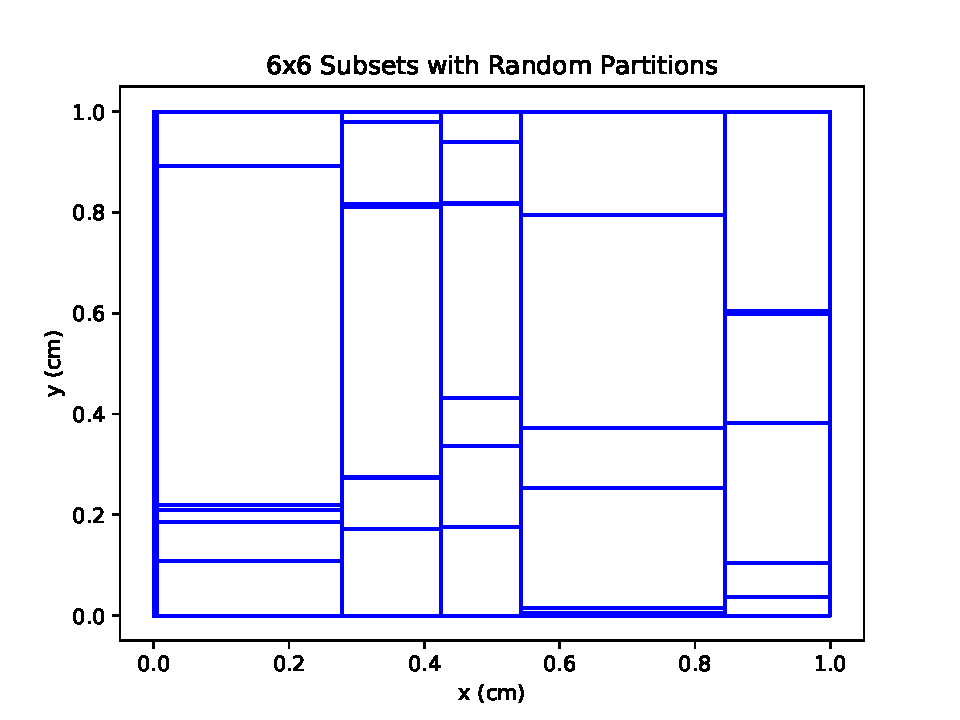
\includegraphics[width=\textwidth]{../cut_line_files/6_random.pdf}
  \caption{6x6 subsets with random partitions.}
  \label{6random}
\end{subfigure}

\begin{subfigure}[b]{0.45\textwidth}
  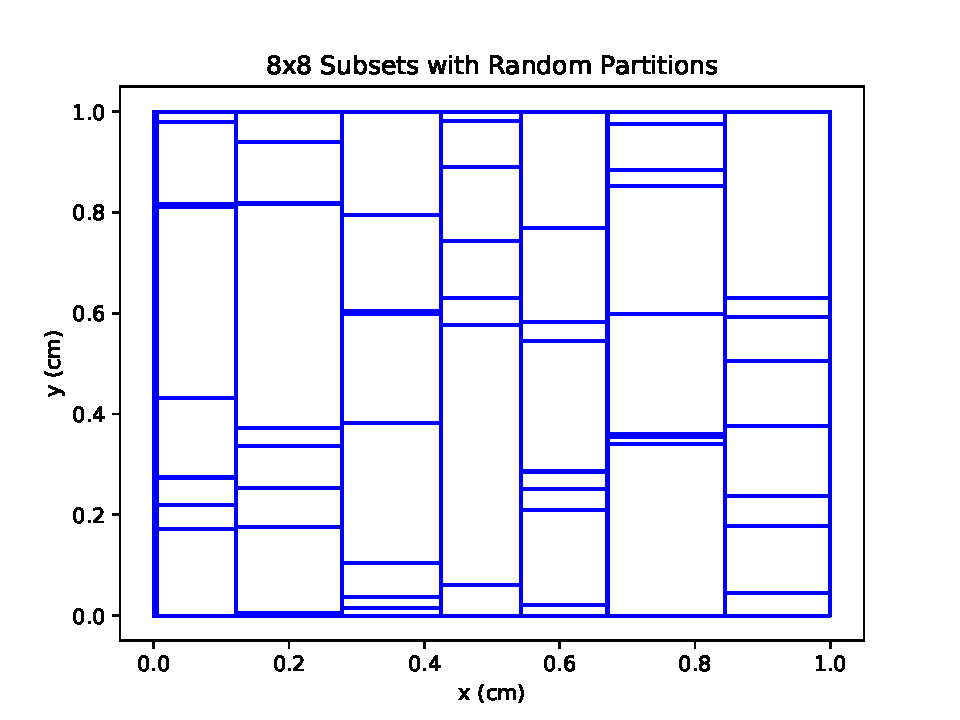
\includegraphics[width=\textwidth]{../cut_line_files/8_random.pdf}
  \caption{8x8 subsets with random partitions.}
  \label{8random}
\end{subfigure}
\begin{subfigure}[b]{0.45\textwidth}
  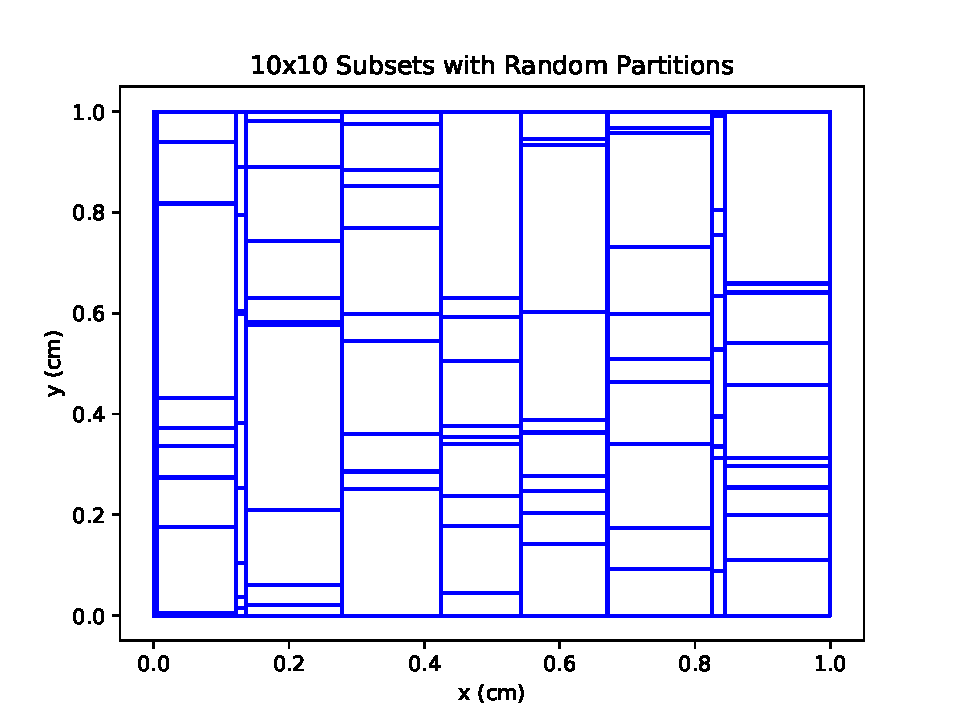
\includegraphics[width=\textwidth]{../cut_line_files/10_random.pdf}
  \caption{10x10 subsets with random partitions.}
  \label{10random}
\end{subfigure}
\caption{Examples of random partitioning.}
\label{random_partitions}
\end{figure}

Using random partitions as shown in Fig. \ref{random_partitions}, the third portion of the 2D verification study was run from 2x2 to 10x10 subsets in x and y and 1 to 6 angles per quadrant.  Figure \ref{random_verification} shows the results of the time-to-solution estimator (solid line) against Ragusa's code (points) for each test case. The time-to-solution estimator verifies perfectly on random partitions with multiple angles per quadrant. 

\begin{figure}[H]
\centering
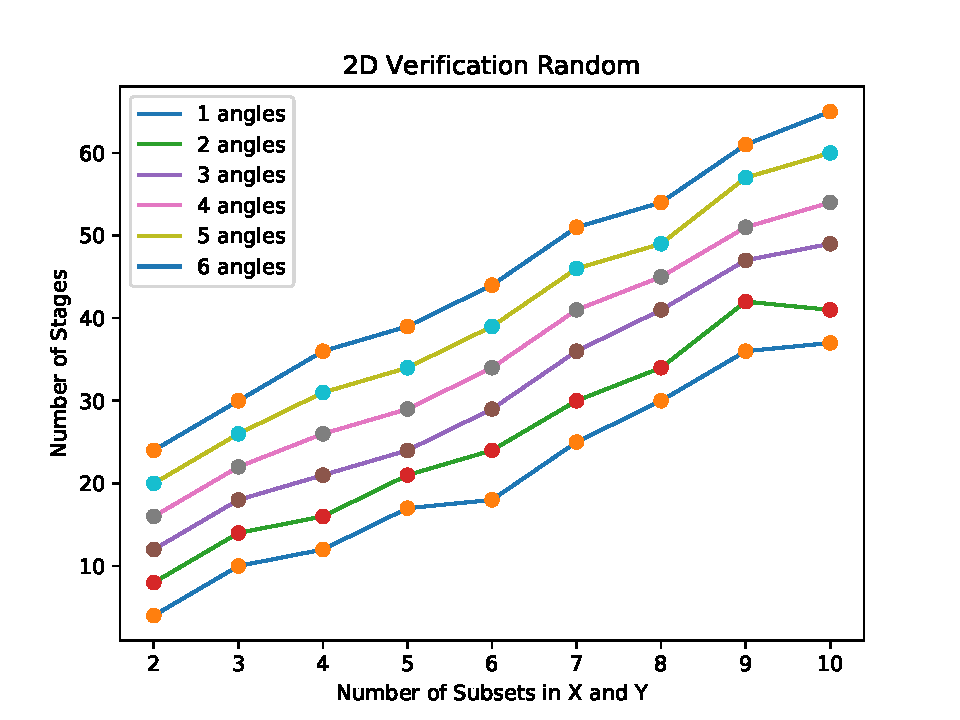
\includegraphics[scale=0.8]{../figures/random_verification.pdf}
\caption{A 2D verification suite with random partitions run from 2x2 to 10x10 subsets with each case being run from 1 to 6 angles per quadrant.}
\label{random_verification}
\end{figure}

\subsection{Probable Worst-Case Partitions}
Figure \ref{worst_partitions} shows four examples of the probable worst-case partitioning scheme used for the final part of the verification study. Cut lines in the x dimension go all the way across the domain, and are uniformly distributed. The cut lines in y are distributed on opposing ends of alternating columns.This reflects a possible partitioning scheme after the load balancing by dimension algorithm described in Section \ref{sec:lbd} is used.
\begin{figure}[H]
\centering
\begin{subfigure}[b]{0.45\textwidth}
  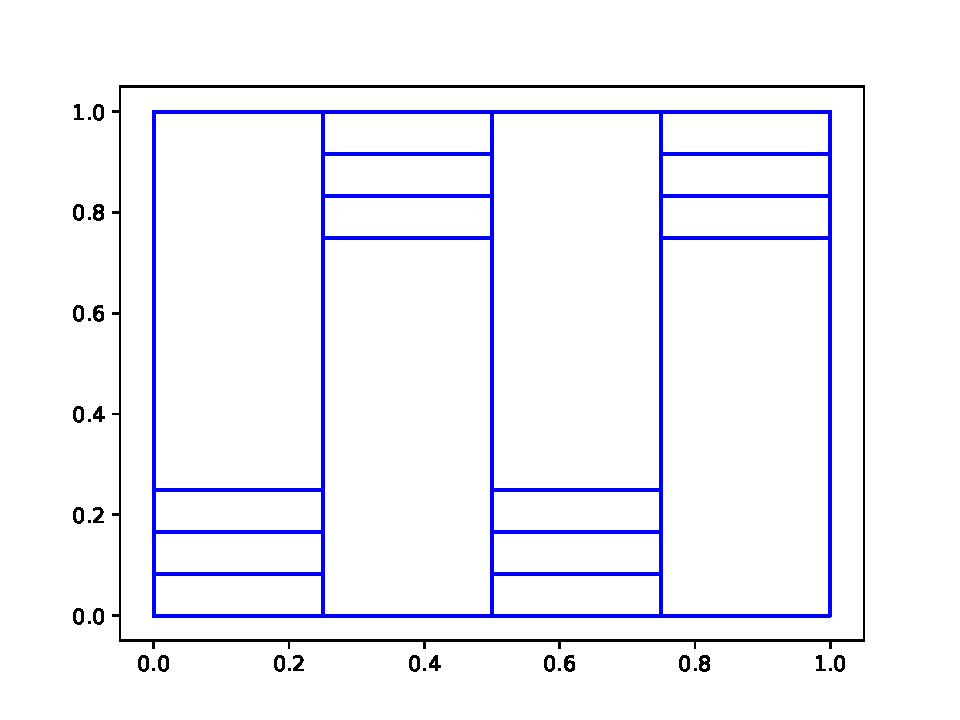
\includegraphics[width=\textwidth]{../cut_line_files/4_worst.pdf}
  \caption{4x4 subsets with probable worst-case partitions.}
  \label{4worst}
\end{subfigure}
\begin{subfigure}[b]{0.45\textwidth}
  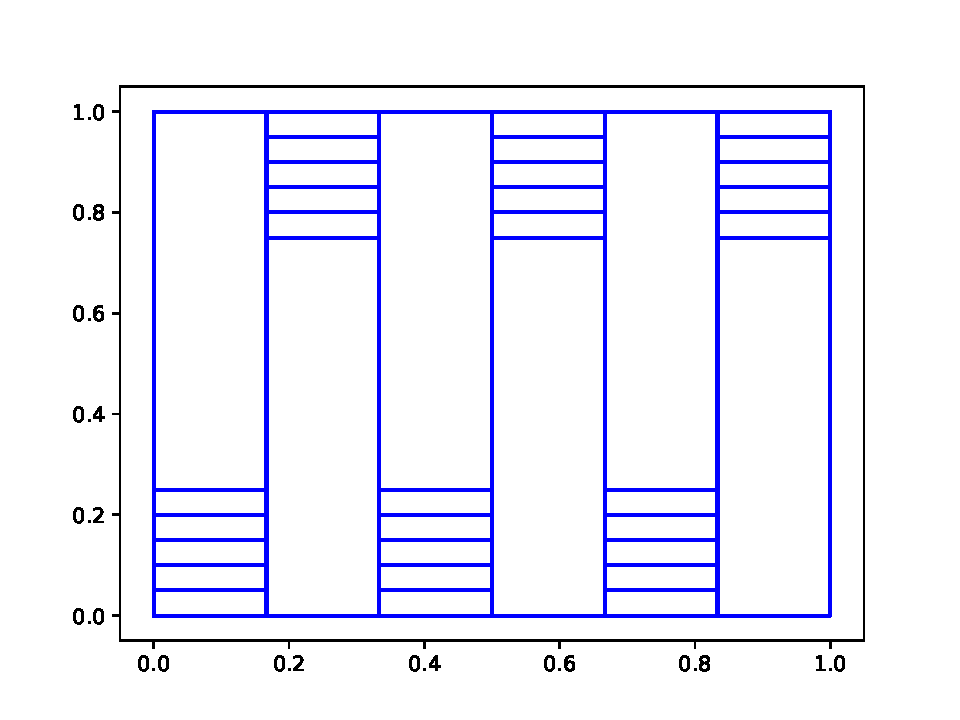
\includegraphics[width=\textwidth]{../cut_line_files/6_worst.pdf}
  \caption{6x6 subsets with probable worst-case partitions.}
  \label{6worst}
\end{subfigure}

\begin{subfigure}[b]{0.45\textwidth}
  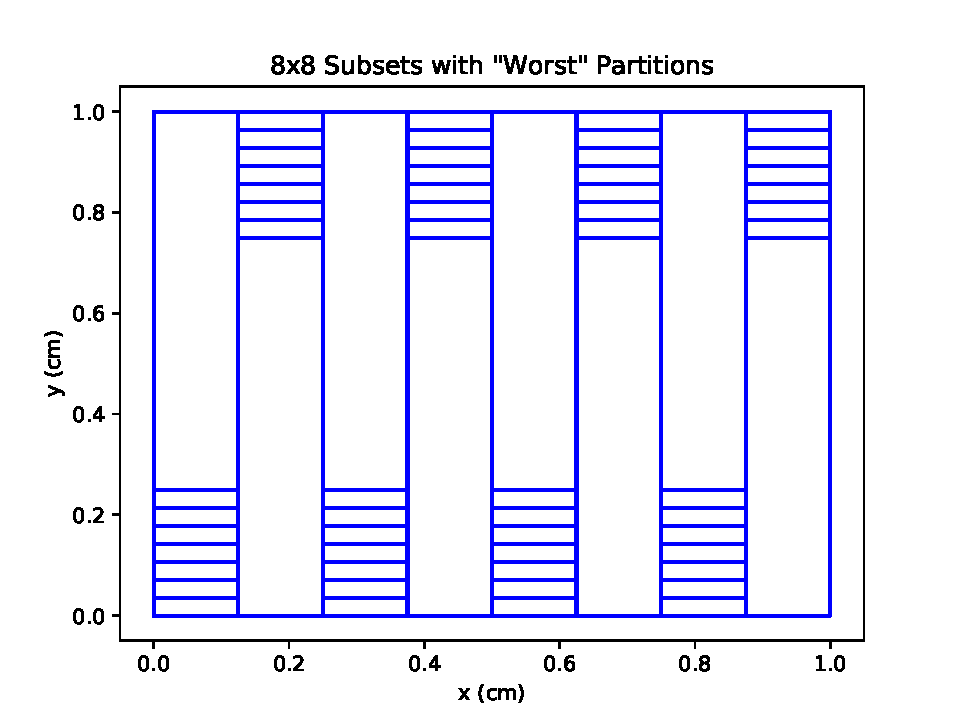
\includegraphics[width=\textwidth]{../cut_line_files/8_worst.pdf}
  \caption{8x8 subsets with probable worst-case partitions.}
  \label{8random}
\end{subfigure}
\begin{subfigure}[b]{0.45\textwidth}
  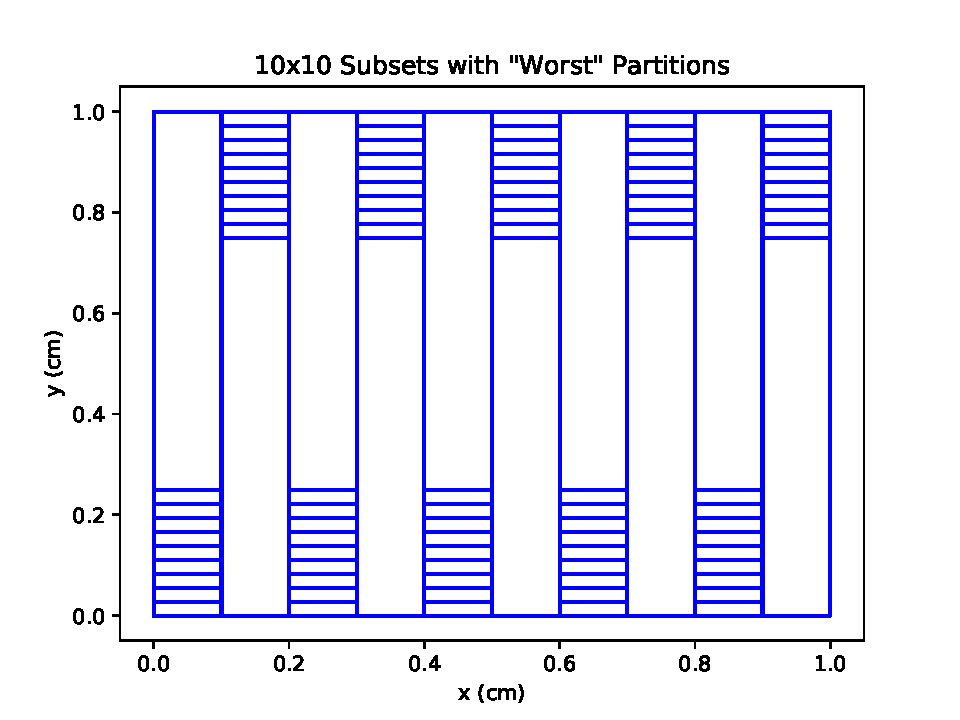
\includegraphics[width=\textwidth]{../cut_line_files/10_worst.pdf}
  \caption{10x10 subsets with probable worst-case partitions.}
  \label{10random}
\end{subfigure}
\caption{Examples of probable worst-case partitioning.}
\label{worst_partitions}
\end{figure}
Using probable worst-case partitions as shown in Fig. \ref{random_partitions}, the final portion of the 2D verification study was run from 2x2 to 10x10 subsets in x and y and 1 to 6 angles per quadrant.  Figure \ref{worst_verification} shows the results of the time-to-solution estimator (solid line) against Ragusa's code (points) for each test case. The time-to-solution estimator verifies perfectly on probable worst-case partitions with multiple angles per quadrant. 
\begin{figure}[H]
\centering
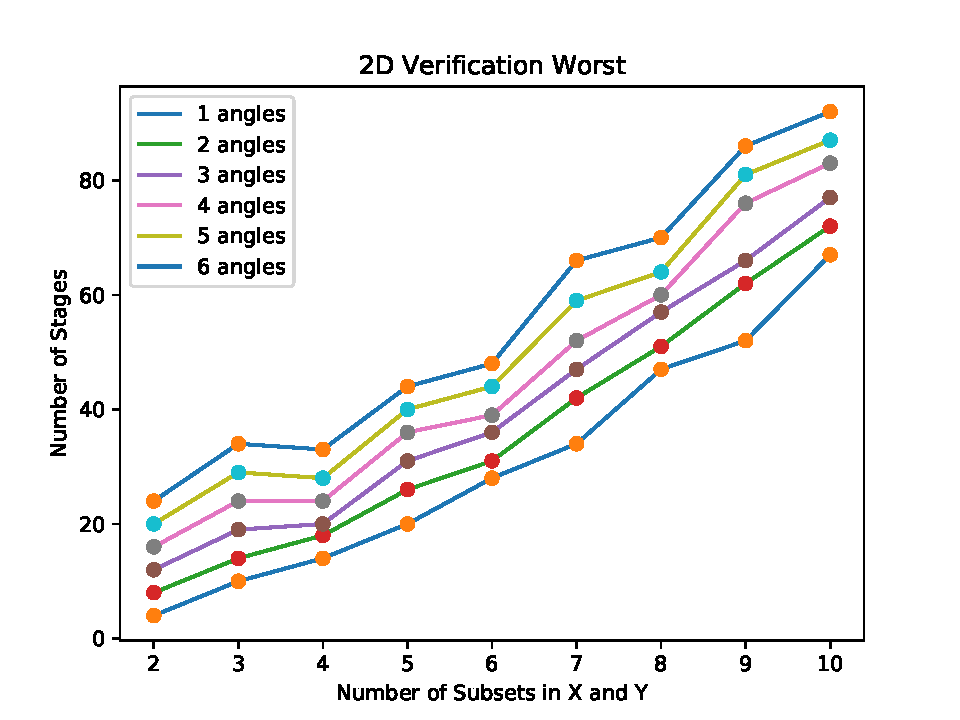
\includegraphics[scale=0.8]{../figures/worst_verification.pdf}
\caption{A 2D verification suite with probable worst-case partitions run from 2x2 to 10x10 subsets with each case being run from 1 to 6 angles per quadrant.}
\label{worst_verification}
\end{figure}

\section{3D Verification}

The 3d verification results will go here.
